\documentclass{article}

\usepackage{arxiv}

\usepackage[utf8]{inputenc} % allow utf-8 input
\usepackage[T1]{fontenc}    % use 8-bit T1 fonts
\usepackage{hyperref}       % hyperlinks
\usepackage{url}            % simple URL typesetting
\usepackage{booktabs}       % professional-quality tables
\usepackage{amsfonts}       % blackboard math symbols
\usepackage{nicefrac}       % compact symbols for 1/2, etc.
\usepackage{microtype}      % microtypography

\usepackage{graphicx}
\usepackage{amsmath}

\newtheorem{definition}{Definition}
\newtheorem{lemma}{Lemma}
\newtheorem{proposition}{Proposition}
\newtheorem{program}{Program}
\newtheorem{convention}{Convention}

\title{Notes on geometrical interpretation of adjoint equation}

%\date{September 9, 1985}	% Here you can change the date presented in the paper title
%\date{} 					% Or removing it

\author{
  Mingli~Yuan \\
  AI Lab \\
  Beijing ColorfulClouds Tech.\\
  Beijing, 100083 \\
  \texttt{mingli.yuan@caiyunapp.com} \\
  %% examples of more authors
  %% \AND
  %% Coauthor \\
  %% Affiliation \\
  %% Address \\
  %% \texttt{email} \\
  %% \And
  %% Coauthor \\
  %% Affiliation \\
  %% Address \\
  %% \texttt{email} \\
  %% \And
  %% Coauthor \\
  %% Affiliation \\
  %% Address \\
  %% \texttt{email} \\
}

% Uncomment to remove the date
%\date{}

% Uncomment to override  the `A preprint' in the header
%\renewcommand{\headeright}{Technical Report}
%\renewcommand{\undertitle}{Technical Report}

\begin{document}
\maketitle

\begin{abstract}
Traditionally, adjoint equation was introduced via the technic of integration-by-part.
After recalling the geometrical interpretation of adjoint in linear cases,
we reveal that adjoint equation shares the same interpretation,
and then a new dual-number-based definition of adjoint equation and proof for equivalence between definitions are given.
\end{abstract}

\keywords{adjoint \and adjoint equation \and geometrical interpretation \and dual number}

\section{Introduction}

The concept of adjoint is very fundamental\cite{Daz1953MethodsOM}\cite{Marchuk1995}, and adjoint equation shows its importance in domains of optimal control\cite{Liberzon2012CalculusOV}, sensitivity analysis\cite{hall1983physical}, and data assimilation\cite{Errico1997WhatIA}. Also, recent contribution\cite{Chen2018NeuralOD} shows adjoint equation can play a role in the intersection area of deep learning and differential equations.

In linear cases, there is an apparent geometrical interpretation of adjoint operators, and in this paper, we want to reveal adjoint equation shares the same interpretation.

\subsection{Definition and geometrical interpretation of adjoint operators in linear case}

Formally, we can define a pair of adjoint operators in a dual system.

\begin{figure}[ht]
\centering
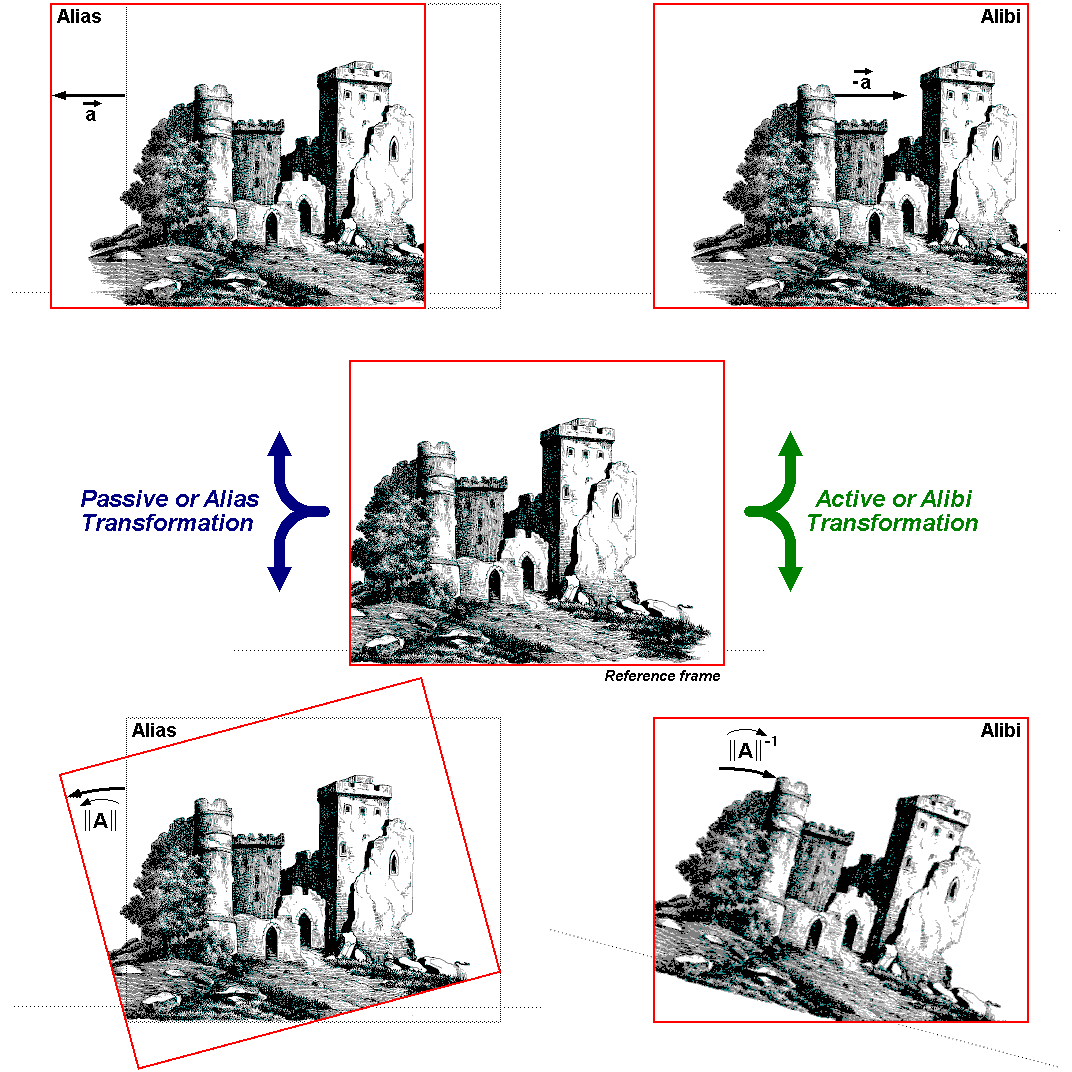
\includegraphics[width=3.5in]{../images/adjoint/alias_and_alibi.png}
\caption{A dual system and two pair of adjoint operators\cite{wiki:aatrans}}
\end{figure}

\begin{definition}
\label{d0}
A dual system $ \langle X, Y \rangle $ is a bilinear mapping $ \langle , \rangle : X \times Y \to F $ where $X$, $Y$ are two vector space and $ F $ is a field.
\end{definition}

\begin{definition}
\label{d1}
For two dual system $ \langle X_1, Y_1 \rangle $ and $ \langle X_2, Y_2 \rangle $ , each of the two operator $ A : X_1 \to X_2$ and $ B : Y_2 \to Y_1 $ is an adjoint of the other counterpart,
if and only if, the equation $$ \langle A \phi, \psi \rangle = \langle \phi, B \psi \rangle $$ holds for arbitrary $ \phi \in X_1 $ and $ \psi \in Y_2 $
\end{definition}

Geometrically, We can interpret $ X $ in $ \langle X, Y \rangle $ as bottom space, while $ Y $ is frame space, and the value of $ \langle x, y \rangle $ is a coordinate.
Under this interpretation, a pair of adjoint operators are just active and passive transformations (or alibi and alias transformations)\cite{wiki:aptrans}.

\subsection{Different problems leading to adjoint equation}

Adjoint equation is a tool when we seek an optimized solution bounded to an evolutionary differential equation, here the optimized solution can be a boundary value to apply control, or instead, an initial value to fit observations aftermath, or possibly, better parameters to influence the process.
Here, we will show some typical problems leading to adjoint equation.

\subsubsection{optimized boundary-value problem}

we need to optimize the boundary value $ \mathbf{u} = \mathbf{y}_{\partial} $ to minimize the error between $ \mathbf{y}_1 = \mathbf{y}(\mathbf{x}, 1)$ and target $ \mathbf{y}_1^o $.

$$
\begin{array}{rcll}
\min &~& J(\mathbf{y_1}, \mathbf{y}_1^o, \mathbf{u}) & \\
\mathrm{s.t.} &~& \dot{\mathbf{y}} = f(\mathbf{x}, t; \theta) & (\mathbf{x}, t) \in \Omega \times [0, 1] \\
&~& \mathbf{y} = u(\mathbf{x}, t; \theta) & (\mathbf{x}, t) \in \partial \Omega \times [0, 1] \\
&~& \mathbf{y}(\mathbf{x}, 0) = \mathbf{y}_0(\mathbf{x}) & \mathbf{x} \in \Omega
\end{array}
$$

And $ J $ is determined by

$$
J(\mathbf{y_1}, \mathbf{y}_1^o, \mathbf{u}) = \frac{1}{2} \int\limits_{\Omega}|\mathbf{y_1} - \mathbf{y_1^o}|^2dx +  \frac{\lambda}{2} \int\limits_{0}^{1}\int\limits_{\partial \Omega} |\mathbf{u}|^2 dS(x) dt
$$

\subsubsection{optimized initial-value problem}

Let $ O(\mathbf{x}, t) $ to be the character functions of the observable area
$$
O(\mathbf{x}, t) = \begin{cases}
1, & \text{if }\mathbf{x}\text{ is observable at t} \\
0, & \text{if }\mathbf{x}\text{ is not observable at t}
\end{cases}
$$

Let $ \mathbf{y} $ to be the status of observable and $ M(\mathbf{x}, \mathbf{y}) $ is a measure method gives the measured value.

At any time $ t $, we have measured value over an observable area:

$$ \mathbf{m}_t = M(\mathbf{x}, \mathbf{y}_t) O(\mathbf{x}, t) $$

we need to optimize the initial value $ \mathbf{u} = \mathbf{y}_0 - \mathbf{y}_0^b $  to minimize the error between the computed measurement $ \mathbf{m}_1 $ and the observed measurement $ \mathbf{m}_1^o $.

$$
\begin{array}{rcll}
\min &~& J(\mathbf{m_1}, \mathbf{m}_1^o, \mathbf{u}) & \\
\mathrm{s.t.} &~& \dot{\mathbf{y}} = f(\mathbf{x}, t; \theta) & (\mathbf{x}, t) \in \Omega \times [0, 1] \\
&~& \mathbf{y} = g(\mathbf{x}, t; \theta) & (\mathbf{x}, t) \in \partial \Omega \times [0, 1] \\
\end{array}
$$

And $ J $ is determined by

$$
J(\mathbf{m_1}, \mathbf{m}_1^o, \mathbf{u}) = \frac{1}{2} \int\limits_{\Omega}|\mathbf{m}_1 - \mathbf{m}_1^o|^2 dx + \frac{\lambda}{2} \int\limits_{\Omega}|\mathbf{u}|^2 dx
$$

\subsubsection{optimized parameter problem}

$$
\begin{array}{rcll}
\min &~& J(\mathbf{y_1}, \mathbf{y}_1^o) & \\
\mathrm{s.t.} &~& \dot{\mathbf{y}} = f(\mathbf{x}, t; \theta) & (\mathbf{x}, t) \in \Omega \times [0, 1] \\
&~& \mathbf{y} = g(\mathbf{x}, t; \theta) & (\mathbf{x}, t) \in \partial \Omega \times [0, 1] \\
&~& \mathbf{y}(\mathbf{x}, 0) = \mathbf{y}_0(\mathbf{x}) & \mathbf{x} \in \Omega
\end{array}
$$

\subsection{The traditional way to introduce adjoint equation}


\section{Geometrical interpretation of adjoint equation}

\subsection{Additional and multiplicational point of view}

\subsection{Forward and backward propagation of a disturbance}

\subsection{The geometrical interpretation}


\section{Reformulate with dual number}


\section{Reformulate disturbance as a space}

the orbit of a disturbance is a point

\section{Applications}

\bibliographystyle{unsrt}
\bibliography{references}

\end{document}
